\documentclass[32pt,aspectratio=169]{beamer}

\usepackage[utf8]{inputenc} % Character encoding, choose your machine's default 
                              % encoding; latin1 or utf8. If you want it read by
                              % others choose latin1
\pdfinfo{
   /Author (Bashar Dudin)
   /Title  (Project Scheduling)
   /Subject (Networks and Flows on Graphs)
}

\usepackage{./Style/My_Beamer} % This is my Beamer style.
\usepackage{./Style/Mystyle} % This is my own defined commands

%----------------------------------------------------------------------------------------
%   TITLE PAGE
%----------------------------------------------------------------------------------------

\author[BD]{Bashar Dudin}

\institute[]{EPITA}
 
\title{Networks and Flows on Graphs} % 
\subtitle{Project Scheduling}

\begin{document}

\begin{frame}[plain]
\titlepage % Print the title page as the first slide
\end{frame}

\begin{frame}{What Is It About ?}
  \begin{halfshyblock}{A Project Scheduling Problem}
    We're confronted with a project scheduling (or planning) problem
    if, in order to achieve an \emph{objective}, we need to go through
    a set of \emph{tasks}, each having limited \emph{ressources} and
    the set of which is subject to a number of \emph{constraints}.
  \end{halfshyblock}
  \pause
  \begin{itemize}
  \item \emph{Tasks} can only be defined once you know what you are
    dealing with, the hard part is to make full sense of how you
    decompose your project into tasks
  \item \emph{Ressources} are generally thought of as the needed time
    for a task to be accomplished, it can also be funds, the number of
    needed employees, etc ...
  \item \emph{Constraints} are grouped into three big types :
    \emph{potential constraints}, \emph{disjunctive constraints} and
    \emph{cumulative constraints}. 
  \end{itemize}
\end{frame}

\begin{frame}{Types of Constraints}
  \textbf{Potential constraints}
  \begin{paremph}
    \begin{itemize}
    \item[] These are \emph{precedence constraints} and
      \emph{constraints of temporal position}. The former correspond
      to constraints of type : ``for task $B$ to start task $A$ has to
      be finished'' ; these are about the order
      in which tasks take place. The constraints of temporal position
      correspond to constraints of type : ``task $A$ cannot start
      before January, $2$''. Mathematically, they are modeled
      identically.
    \end{itemize}
  \end{paremph}
  \textbf{Disjunctive constraints}
  \begin{paremph}
    \begin{itemize}
    \item[] These are constraints of type : ``tasks $A$ and $B$ cannot
      happen simultaneously''.
    \end{itemize}
  \end{paremph}
  \textbf{Cumulative constraints}
  \begin{paremph}
    \begin{itemize}
    \item[] These are relative to the evolution
        of resources needed to accomplish a task. They are generally
        hard to model.
      \end{itemize}
  \end{paremph}
\end{frame}

\begin{frame}{Types of Constraints}
  \textbf{Potential constraints}
  \begin{paremph}
    \begin{itemize}
    \item[] These are \emph{precedence constraints} and
      \emph{constraints of temporal position}. The former correspond
      to constraints of type : ``for task $B$ to start task $A$ has to
      be finished'' ; these are about the order
      in which tasks take place. The constraints of temporal position
      correspond to constraints of type : ``task $A$ cannot start
      before January, $2$''. Mathematically, they are modeled
      identically.
    \end{itemize}
  \end{paremph}
  \color{lightgray}{
  \textbf{Disjunctive constraints}
  \begin{paremph}[lightgray]
    \begin{itemize}
    \item[] \color{lightgray}{These are constraints of type : ``tasks $A$ and $B$ cannot
      happen simultaneously''.}
    \end{itemize}
  \end{paremph}
  \textbf{Cumulative constraints}
  \begin{paremph}[lightgray]
    \begin{itemize}
    \item[] \color{lightgray}{These are relative to the evolution
        of resources needed to accomplish a task. They are generally
        hard to model.}
      \end{itemize}
  \end{paremph}
  }
\end{frame}

\begin{frame}{What Are We Looking for ?}
  There are three things we're interested in when dealing with
  scheduling problems (assuming we only have potential constraints)
  \begin{itemize}
  \item<1-> earliest dates at which tasks can start
  \item<2-> latest dates ; once the minimum date has been computed
  \item<3-> margins, i.e. the difference between latest and earliest
    date of a task.
  \end{itemize}
  \pause[4]
  We shall working two standard approaches aiming at answering these
  $3$ related questions : the MPM method (the french method) and PERT
  method (the american one).
\end{frame}

\begin{frame}{Scheduling methods}
   \textbf{MPM (Meta Potential Method)}
  \begin{paremph}
    \begin{itemize}
    \item[] In the MPM approach tasks are understood as vertices of a
      graph, whose arrows correspond to precedence constraints. Each
      arrow is valued by a number representing the time between the
      start of its origin till the start of its target.
    \end{itemize}
  \end{paremph}
  \pause
  \textbf{PERT (Program Evaluation and Review Technique)}
  \begin{paremph}
    \begin{itemize}
    \item[] In the PERT case, the tasks are represented by arrows,
      while vertices should be understood as intermediate achievements
      attained once a task is completed. An arrow is valued by the
      time the corresponding task takes. Using a PERT diagram needs
      serious work on the chosen way of modeling the problem at
      hand. It's advantage in respect to the MPM approach is the fact
      it is better suited when randomness is involved. 
    \end{itemize}
  \end{paremph}
\end{frame}

\begin{frame}
  \frametitle{Working Example}
  Consider a project given by tasks a to g, under the following
  conditions of resource and constraints
  \begin{figure}
    \begin{tabular}{|c|c|c|}
      \hline
      Tasks & Needed Time & Constraints \\
      \hline
      a & $6$ & \\
      \hline
      b & $3$ & \\
      \hline
      c & $6$ & \\
      \hline
      d & $2$ & b accomplished \\
      \hline
      e & $4$ & b accomplished \\
      \hline
      f & $3$ & d and a accomplished \\
      \hline
      g & $1$ & f, e, c accomplished \\
      \hline
    \end{tabular}
  \end{figure}
\end{frame}

\begin{frame}
  \frametitle{Working Example : MPM model}
  \begin{onlyenv}<1>
    Each vertex corresponds to one of the tasks, $s$ and $t$ are start
    and end of project.
    \begin{figure}
      \centering
      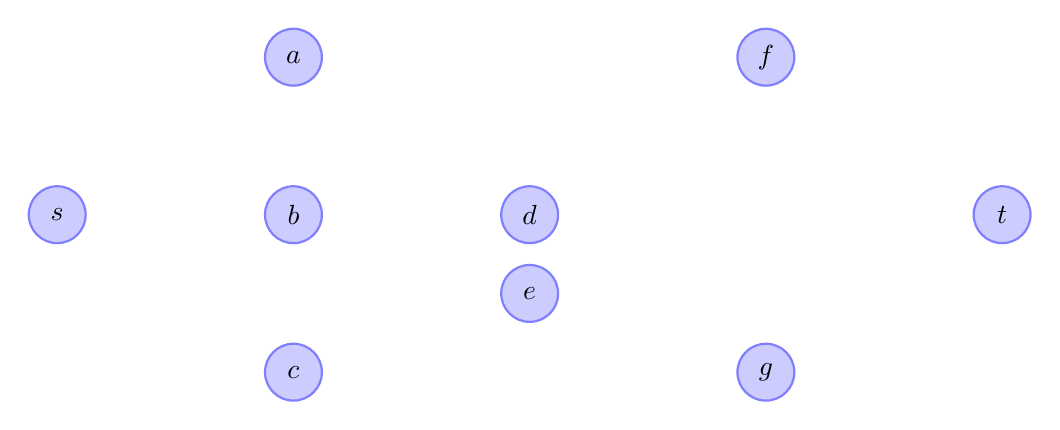
\begin{tikzpicture}
        [minimum width={width("b")+1.5em},
        vertex/.style={circle,draw=blue!50,fill=blue!20,thick},
        arr/.style={->,>=stealth',semithick}]
        \node (s) at (3,5) [vertex] {$s$};
        \node (t) at (15,5) [vertex] {$t$};
        \node (a) at (6,7) [vertex] {$a$};
        \node (b) at (6,5) [vertex] {$b$};
        \node (c) at (6,3) [vertex] {$c$};
        \node (d) at (9,5) [vertex] {$d$};
        \node (e) at (9,4) [vertex] {$e$};
        \node (f) at (12,7) [vertex] {$f$};
        \node (g) at (12,3) [vertex] {$g$};
     \end{tikzpicture}
     \end{figure}
   \end{onlyenv}
   \begin{onlyenv}<2> 
     Arrows give a picture of the potential constraints satisfied by
     the tasks.
     \begin{figure}
      \centering
      \begin{tikzpicture}
        [minimum width={width("b")+1.5em},
        vertex/.style={circle,draw=blue!50,fill=blue!20,thick},
        arr/.style={->,>=stealth',semithick}]
        \node (s) at (3,5) [vertex] {$s$}
           edge[arr] (a)
           edge[arr] (b)
           edge[arr] (c);
        \node (t) at (15,5) [vertex] {$t$};
        \node (a) at (6,7) [vertex] {$a$}
           edge[arr] (f);
        \node (b) at (6,5) [vertex] {$b$}
           edge[arr] (d)
           edge[arr] (e);
        \node (c) at (6,3) [vertex] {$c$}
           edge[arr] (g);
        \node (d) at (9,5) [vertex] {$d$}
           edge[arr] (f);
        \node (e) at (9,4) [vertex] {$e$}
           edge[arr] (g);
        \node (f) at (12,7) [vertex] {$f$}
           edge[arr] (g);
        \node (g) at (12,3) [vertex] {$g$}
           edge[arr] (t);
     \end{tikzpicture}
   \end{figure}
 \end{onlyenv}
 \begin{onlyenv}<3->
   Valuation at arrow is the time laps between start point
   of origin till start point of target.
   \begin{figure}
      \centering
      \begin{tikzpicture}
        [minimum width={width("b")+1.5em},
        vertex/.style={circle,draw=blue!50,fill=blue!20,thick},
        arr/.style={->,>=stealth',semithick}]
        \node (s) at (3,5) [vertex] {$s$}
           edge[arr] node[above, red] {$0$} (a)
           edge[arr] node[above, red] {$0$} (b)
           edge[arr] node[above, red] {$0$} (c);
        \node (t) at (15,5) [vertex] {$t$};
        \node (a) at (6,7) [vertex] {$a$}
           edge[arr] node[above, red] {$6$}(f);
        \node (b) at (6,5) [vertex] {$b$}
           edge[arr] node[above, red] {$3$} (d)
           edge[arr] node[below, red] {$3$} (e);
        \node (c) at (6,3) [vertex] {$c$}
           edge[arr] node[below, red] {$6$} (g);
        \node (d) at (9,5) [vertex] {$d$}
           edge[arr] node[above, red] {$2$} (f);
        \node (e) at (9,4) [vertex] {$e$}
           edge[arr] node[above, red] {$3$} (g);
        \node (f) at (12,7) [vertex] {$f$}
           edge[arr] node[right, red] {$3$} (g);
        \node (g) at (12,3) [vertex] {$g$}
           edge[arr] node[above, red] {$1$} (t);
     \end{tikzpicture}
   \end{figure}
 \end{onlyenv}
\end{frame}

\begin{frame}
  \frametitle{Working Example : MPM / Earliest Dates}
  \begin{columns}
    \begin{column}{.6\textwidth}
      
      \vspace{.2\baselineskip}
      The point is to compute the earliest date at which the project
      ends. 
      
      \vspace{.3\baselineskip}
      This is governed by paths from source to target that take
      the longest time. These are called \emph{critical
        paths}, the name comes from the fact any delay $\varepsilon$
      in tasks along this path would delay the whole project by
      $\varepsilon$.

      \vspace{.3\baselineskip} 
      Our goal can be achieved by adapting Ford's algorithms to look
      for longest paths in our graph.
      
      \vspace{.3\baselineskip}
      \begin{alertblock}{Beware}
        For this strategy to work, it is
        important to have graphs without circuits! in our case that
        would mean there are contradicting tasks ...
      \end{alertblock}
    \end{column}
    \begin{column}{.4\textwidth}
      \begin{onlyenv}<1>
        \begin{figure}
          \begin{tikzpicture}
            [scale= .9, minimum width={width("b")+1.5em},
            vertex/.style={circle,draw=blue!50,fill=blue!20,thick},
            arr/.style={->,>=stealth',semithick}]
            \node (t) at (8,2.5) [vertex] {$t$};
            \node (g) at (6,4) [vertex] {$g$}
            edge[arr] node[below left, red] {$1$} (t)
            ;
            \node (f) at (10,4) [vertex] {$f$}
            edge[arr] node[above, red] {$3$} (g)
            ;
            \node (e) at (7,6) [vertex] {$e$}
            edge[arr] node[right, red] {$3$} (g)
            ;
            \node (d) at (8,6) [vertex] {$d$}
            edge[arr] node[left, red] {$2$} (f)
            ;
            \node (c) at (6,8) [vertex] {$c$}
            edge[arr] node[left, red] {$6$} (g)
            ;
            \node (b) at (8,8) [vertex] {$b$}
            edge[arr] node[right, red] {$3$} (d)
            edge[arr] node[left, red] {$3$} (e)
            ;   
            \node (a) at (10,8) [vertex] {$a$}
            edge[arr] node[right, red] {$6$}(f)
            ;
            \node (s) at (8,10) [vertex] {$s$}
            edge[arr] node[right, red] {$0$} (a)
            edge[arr] node[right, red] {$0$} (b)
            edge[arr] node[right, red] {$0$} (c)
            ;   
         \end{tikzpicture}
       \end{figure}
      \end{onlyenv}
    \end{column}
  \end{columns}
\end{frame}

\begin{frame}
  \frametitle{Working Example : MPM / Earliest Dates}
  \begin{columns}
    \begin{column}{.6\textwidth}
      The point is to compute the earliest date at which the project
      ends. 
      
      \vspace{.3\baselineskip}
      This is governed by paths from source to target that take
      the longest time. These are called \emph{critical
        paths}, the name comes from the fact any delay $\varepsilon$
      in tasks along this path would delay the whole project by
      $\varepsilon$.

      \vspace{.3\baselineskip} 
      Our goal can be achieved by adapting Ford's algorithms to look
      for longest paths in our graph.
      
      \vspace{.3\baselineskip}
      \begin{alertblock}{Beware}
        For this strategy to work, it is
        important to have graphs without circuits! in our case that
        would mean there are contradicting tasks ...
      \end{alertblock}
    \end{column}
    \begin{column}{.4\textwidth}
      \begin{onlyenv}<1>
        
        \vspace{.5\baselineskip}
          \begin{tikzpicture}
            [scale= .9, minimum width={width("b")+1.5em},
            vertex/.style={circle,draw=blue!50,fill=blue!20,thick},
            arr/.style={->,>=stealth',semithick}]
            \node (t) at (8,2.5) [vertex, label=0:$10$] {$t$};
            \node (g) at (6,4) [vertex, label=180:$9$] {$g$}
            edge[arr] node[below left, red] {$1$} (t)
            ;
            \node (f) at (10,4) [vertex, label=0:$6$] {$f$}
            edge[arr] node[above, red] {$3$} (g)
            ;
            \node (e) at (7,6) [vertex, label=180:$3$] {$e$}
            edge[arr] node[right, red] {$3$} (g)
            ;
            \node (d) at (8,6) [vertex, label=0:$3$] {$d$}
            edge[arr] node[left, red] {$2$} (f)
            ;
            \node (c) at (6,8) [vertex, label=0:$0$] {$c$}
            edge[arr] node[left, red] {$6$} (g)
            ;
            \node (b) at (8,8) [vertex, label=0:$0$] {$b$}
            edge[arr] node[right, red] {$3$} (d)
            edge[arr] node[left, red] {$3$} (e)
            ;   
            \node (a) at (10,8) [vertex, label=0:$0$] {$a$}
            edge[arr] node[right, red] {$6$}(f)
            ;
            \node (s) at (8,10) [vertex, label=0:$0$] {$s$}
            edge[arr] node[right, red] {$0$} (a)
            edge[arr] node[right, red] {$0$} (b)
            edge[arr] node[right, red] {$0$} (c)
            ;   
         \end{tikzpicture}
      \end{onlyenv}
    \end{column}
  \end{columns}
\end{frame}

\begin{frame}
  \frametitle{Working Example : MPM / Earliest Dates}
  \begin{columns}
    \begin{column}{.6\textwidth}
      The earliest date at which to expect our project is accomplished
      is $10$ time units from our starting date.

      \vspace{.3\baselineskip} 
      More generally, we have computed the earliest date at which to
      expect any task to start. The start $t$ which correspond to the
      end of the project starts at $10$.

      \vspace{.3\baselineskip}
      All \emph{critical paths} from source to target are the
      (elementary) ones contained in the subgraph in green. There is
      only one here.
    \end{column}
    \begin{column}{.4\textwidth}
      \begin{onlyenv}<1>
        
        \vspace{.5\baselineskip}
          \begin{tikzpicture}
            [scale= .9, minimum width={width("b")+1.5em},
            vertex/.style={circle,draw=blue!50,fill=blue!20,thick},
            vertexg/.style={circle,draw=green!50!black,fill=green!10,thick},
            arr/.style={->,>=stealth',semithick}]
            \node (t) at (8,2.5) [vertexg, label=0:$10$] {$t$};
            \node (g) at (6,4) [vertexg, label=180:$9$] {$g$}
            edge[arr, green!50!black, very thick] node[below left, red] {$1$} (t)
            ;
            \node (f) at (10,4) [vertexg, label=0:$6$] {$f$}
            edge[arr, green!50!black, very thick] node[above, red] {$3$} (g)
            ;
            \node (e) at (7,6) [vertex, label=180:$3$] {$e$}
            edge[arr] node[right, red] {$3$} (g)
            ;
            \node (d) at (8,6) [vertex, label=0:$3$] {$d$}
            edge[arr] node[left, red] {$2$} (f)
            ;
            \node (c) at (6,8) [vertex, label=0:$0$] {$c$}
            edge[arr] node[left, red] {$6$} (g)
            ;
            \node (b) at (8,8) [vertex, label=0:$0$] {$b$}
            edge[arr] node[right, red] {$3$} (d)
            edge[arr] node[left, red] {$3$} (e)
            ;   
            \node (a) at (10,8) [vertexg, label=0:$0$] {$a$}
            edge[arr, green!50!black, very thick] node[right, red] {$6$}(f)
            ;
            \node (s) at (8,10) [vertexg, label=0:$0$] {$s$}
            edge[arr, green!50!black, very thick] node[right, red] {$0$} (a)
            edge[arr] node[right, red] {$0$} (b)
            edge[arr] node[right, red] {$0$} (c)
            ;   
         \end{tikzpicture}
      \end{onlyenv}
    \end{column}
  \end{columns}
\end{frame}

\begin{frame}
  \frametitle{Working Example : MPM / Latest Dates}
  \begin{columns}
    \begin{column}{.6\textwidth}
      Knowing that the project, at the earliest, ends $10$ time units
      after it starts, we can compute the latest dates at which
      non-critical tasks can start. 
      
      \vspace{.3\baselineskip}
      To do so, one looks for lengths of \emph{shortest} paths
      starting at $t$ with valuation $10$.      
      
      \begin{uncoverenv}<0>
      \vspace{.3\baselineskip} 
      We get the graph on the right. Each vertex is valued by the
      latest date at which it can start, keeping the project ending
      time at $10$.

      \vspace{.3\baselineskip}
      Notice that valuation of the critical path do not change.
      \end{uncoverenv}
    \end{column}
    \begin{column}{.4\textwidth}
      \begin{onlyenv}<1>
        
        \vspace{.5\baselineskip}
          \begin{tikzpicture}
            [scale= .9, minimum width={width("b")+1.5em},
            vertex/.style={circle,draw=blue!50,fill=blue!20,thick},
            vertexg/.style={circle,draw=green!50!black,fill=green!10,thick},
            arr/.style={->,>=stealth',semithick}]
            \node (t) at (8,2.5) [vertexg, label=0:$10$] {$t$};
            \node (g) at (6,4) [vertexg, label=180:$$] {$g$}
            edge[arr, green!50!black, very thick] node[below left, red] {$1$} (t)
            ;
            \node (f) at (10,4) [vertexg, label=0:$$] {$f$}
            edge[arr, green!50!black, very thick] node[above, red] {$3$} (g)
            ;
            \node (e) at (7,6) [vertex, label=180:$$] {$e$}
            edge[arr] node[right, red] {$3$} (g)
            ;
            \node (d) at (8,6) [vertex, label=0:$$] {$d$}
            edge[arr] node[left, red] {$2$} (f)
            ;
            \node (c) at (6,8) [vertex, label=0:$$] {$c$}
            edge[arr] node[left, red] {$6$} (g)
            ;
            \node (b) at (8,8) [vertex, label=0:$$] {$b$}
            edge[arr] node[right, red] {$3$} (d)
            edge[arr] node[left, red] {$3$} (e)
            ;   
            \node (a) at (10,8) [vertexg, label=0:$$] {$a$}
            edge[arr, green!50!black, very thick] node[right, red] {$6$}(f)
            ;
            \node (s) at (8,10) [vertexg, label=0:$$] {$s$}
            edge[arr, green!50!black, very thick] node[right, red] {$0$} (a)
            edge[arr] node[right, red] {$0$} (b)
            edge[arr] node[right, red] {$0$} (c)
            ;   
         \end{tikzpicture}
      \end{onlyenv}
    \end{column}
  \end{columns}
\end{frame}

\begin{frame}
  \frametitle{Working Example : MPM / Latest Dates}
  \begin{columns}
    \begin{column}{.6\textwidth}
      Knowing that the project, at the earliest, ends $10$ time units
      after it starts, we can compute the latest dates at which
      non-critical tasks can start. 
      
      \vspace{.3\baselineskip}
      To do so, one looks for lengths of \emph{shortest} paths
      starting at $t$ with valuation $10$.      

      \vspace{.3\baselineskip} 
      We get the graph on the right. Each vertex is valued by the
      latest date at which it can start, keeping the project ending
      time at $10$.

      \vspace{.3\baselineskip}
      Notice that valuation of the critical path do not change. 
    \end{column}
    \begin{column}{.4\textwidth}
      \begin{onlyenv}<1>
        
        \vspace{.5\baselineskip}
          \begin{tikzpicture}
            [scale= .9, minimum width={width("b")+1.5em},
            vertex/.style={circle,draw=blue!50,fill=blue!20,thick},
            vertexg/.style={circle,draw=green!50!black,fill=green!10,thick},
            arr/.style={->,>=stealth',semithick}]
            \node (t) at (8,2.5) [vertexg, label=0:$10$] {$t$};
            \node (g) at (6,4) [vertexg, label=180:$9$] {$g$}
            edge[arr, green!50!black, very thick] node[below left, red] {$1$} (t)
            ;
            \node (f) at (10,4) [vertexg, label=0:$6$] {$f$}
            edge[arr, green!50!black, very thick] node[above, red] {$3$} (g)
            ;
            \node (e) at (7,6) [vertex, label=180:$6$] {$e$}
            edge[arr] node[right, red] {$3$} (g)
            ;
            \node (d) at (8,6) [vertex, label=0:$4$] {$d$}
            edge[arr] node[left, red] {$2$} (f)
            ;
            \node (c) at (6,8) [vertex, label=0:$3$] {$c$}
            edge[arr] node[left, red] {$6$} (g)
            ;
            \node (b) at (8,8) [vertex, label=0:$1$] {$b$}
            edge[arr] node[right, red] {$3$} (d)
            edge[arr] node[left, red] {$3$} (e)
            ;   
            \node (a) at (10,8) [vertexg, label=0:$0$] {$a$}
            edge[arr, green!50!black, very thick] node[right, red] {$6$}(f)
            ;
            \node (s) at (8,10) [vertexg, label=0:$0$] {$s$}
            edge[arr, green!50!black, very thick] node[right, red] {$0$} (a)
            edge[arr] node[right, red] {$0$} (b)
            edge[arr] node[right, red] {$0$} (c)
            ;   
         \end{tikzpicture}
      \end{onlyenv}
    \end{column}
  \end{columns}
\end{frame}

\begin{frame}
  \frametitle{Working Example : MPM / Margins}
  \begin{columns}
    \begin{column}{.6\textwidth}

      The margin at a vertex is simply the difference between the
      latest date to start and the earliest one.

      \vspace{.3\baselineskip}
      Notice that along the critical path, margins are $0$. 
    \end{column}
    \begin{column}{.4\textwidth}
      \begin{onlyenv}<1>
        
        \vspace{.5\baselineskip}
          \begin{tikzpicture}
            [scale= .9, minimum width={width("b")+1.5em},
            vertex/.style={circle,draw=blue!50,fill=blue!20,thick},
            vertexg/.style={circle,draw=green!50!black,fill=green!10,thick},
            arr/.style={->,>=stealth',semithick}]
            \node (t) at (8,2.5) [vertexg, label=0:$0$] {$t$};
            \node (g) at (6,4) [vertexg, label=180:$0$] {$g$}
            edge[arr, green!50!black, very thick] node[below left, red] {$1$} (t)
            ;
            \node (f) at (10,4) [vertexg, label=0:$0$] {$f$}
            edge[arr, green!50!black, very thick] node[above, red] {$3$} (g)
            ;
            \node (e) at (7,6) [vertex, label=180:$3$] {$e$}
            edge[arr] node[right, red] {$3$} (g)
            ;
            \node (d) at (8,6) [vertex, label=0:$1$] {$d$}
            edge[arr] node[left, red] {$2$} (f)
            ;
            \node (c) at (6,8) [vertex, label=0:$3$] {$c$}
            edge[arr] node[left, red] {$6$} (g)
            ;
            \node (b) at (8,8) [vertex, label=0:$1$] {$b$}
            edge[arr] node[right, red] {$3$} (d)
            edge[arr] node[left, red] {$3$} (e)
            ;   
            \node (a) at (10,8) [vertexg, label=0:$0$] {$a$}
            edge[arr, green!50!black, very thick] node[right, red] {$6$}(f)
            ;
            \node (s) at (8,10) [vertexg, label=0:$0$] {$s$}
            edge[arr, green!50!black, very thick] node[right, red] {$0$} (a)
            edge[arr] node[right, red] {$0$} (b)
            edge[arr] node[right, red] {$0$} (c)
            ;   
         \end{tikzpicture}
      \end{onlyenv}
    \end{column}
  \end{columns}
\end{frame}

\begin{frame}
  \frametitle{Working Example : The PERT approach}
  Recall that in the PERT approach, tasks give rise to arrows valued
  by the time a task needs to be accomplished. Vertices correspond to
  intermediate objectives ; defining them comes, at first, from the
  concrete situation at hand. 

  \vspace{.3\baselineskip}
  In our case, starting from a vertex $5$ corresponding to project
  end, we can define vertex $4$ as $f$, $c$, $e$ are accomplished etc
  ... This is arguably a ``mathematician'' example.
  \begin{figure}
    \centering
    \begin{tikzpicture}
        [scale=.85, minimum width={width("b")+1.5em},
        vertex/.style={circle,draw=blue!50,fill=blue!20,thick},
        arr/.style={->,>=stealth',semithick}]
        \node (5) at (13,5) [vertex] {$5$};
        \node (4) at (9,5) [vertex] {$4$}
           edge[arr] node[above, red] {$g\,\, [1]$} (5);
        \node (3) at (6,3) [vertex] {$3$}
           edge[arr] node[below, red] {$e\,\, [4]$} (4);
        \node (2) at (6,7) [vertex] {$2$}
           edge[arr] node[above, red] {$f\,\, [3]$}(4);
        \node (1) at (3,5) [vertex] {$1$}
           edge[arr] node[above, red] {$a\,\, [6]$} (2)
           edge[arr] node[above, red] {$c\,\, [6]$} (4)
           edge[arr] node[above, red] {$b\,\, [3]$} (3);
     \end{tikzpicture}
  \end{figure}
\end{frame}{}

\begin{frame}
  \centering
{\Large \textbf{This is it for the course on Graphs, Networks and Flows.\\
    Good luck with your final exams!}}
\end{frame}


%%%%%%%%%%%%%%%%%%%%%%%%%%%%%%%%%%%%%%%%%%%%%%%%%%%%%%%%%%%%%%%

\end{document}

%%% Local Variables:
%%% mode: latex
%%% TeX-master: t
%%% End:
